%============================================================
% RESULTS
%============================================================

\section{Results}
\label{sec:results}

%============================================================
\subsection{Data Preparation and Quality Assessment}
%============================================================

The final analytical dataset contained 401 observations with
information on age and baseline headache frequency. Headache
frequency was treated as a count variable representing the number of
headache days during the baseline period.

Initial inspection identified five observations with non-integer
headache-frequency values. These observations were 10.67, 18.67,
26.67, 22.67, and 26.67 days. Because the Poisson distribution is
defined for integer-valued counts, the five values were rounded to
the nearest whole number before fitting the models. No missing
observations were identified for age or headache frequency.

Following data preparation, headache frequency ranged from 3 to
28 days.

\begin{table}[H]
\centering
\caption{Non-integer headache-frequency observations identified during data preparation}
\label{tab:noninteger}
\begin{tabular}{rr}
\toprule
Age & Original Frequency \\
\midrule
23 & 10.67 \\
36 & 18.67 \\
28 & 26.67 \\
23 & 22.67 \\
33 & 26.67 \\
\bottomrule
\end{tabular}
\end{table}

%============================================================
\subsection{Descriptive Analysis}
%============================================================

The mean baseline headache frequency was 16.18 days, with a
standard deviation of 6.71 days. The median was 15 days, and the
observed values ranged from 3 to 28 days.

\begin{table}[H]
\centering
\caption{Descriptive statistics for baseline headache frequency}
\label{tab:descriptive}
\begin{tabular}{lr}
\toprule
Statistic & Value \\
\midrule
Sample size & 401 \\
Mean & 16.18 \\
Variance & 44.98 \\
Standard deviation & 6.71 \\
Median & 15.00 \\
Minimum & 3.00 \\
Maximum & 28.00 \\
Variance-to-mean ratio & 2.78 \\
\bottomrule
\end{tabular}
\end{table}

The variance was considerably larger than the mean, indicating
substantial variability in headache frequency between patients.

%============================================================
\subsection{Assessment of Over-dispersion}
%============================================================

Under a standard Poisson model, the mean and variance are expected
to be equal. For the present data, the estimated mean was 16.18 and
the estimated variance was 44.98. The resulting variance-to-mean
ratio was

\[
\frac{\operatorname{Var}(Y)}{E(Y)}
=
\frac{44.98}{16.18}
=
2.78.
\]

The ratio was substantially greater than one, indicating
over-dispersion relative to the standard Poisson assumption. This
provided a clear reason to investigate models that could account for
heterogeneity between patients.

%============================================================
\subsection{NPMLE Gradient-Function Analysis}
%============================================================

A nonparametric maximum likelihood estimate (NPMLE) was obtained
using the CAMAN package as an exploratory analysis of the underlying
mixing distribution. The NPMLE was estimated using the VEM algorithm
followed by EM refinement.

The resulting gradient function is shown in
Figure~\ref{fig:gradient}.

\begin{figure}[H]
\centering
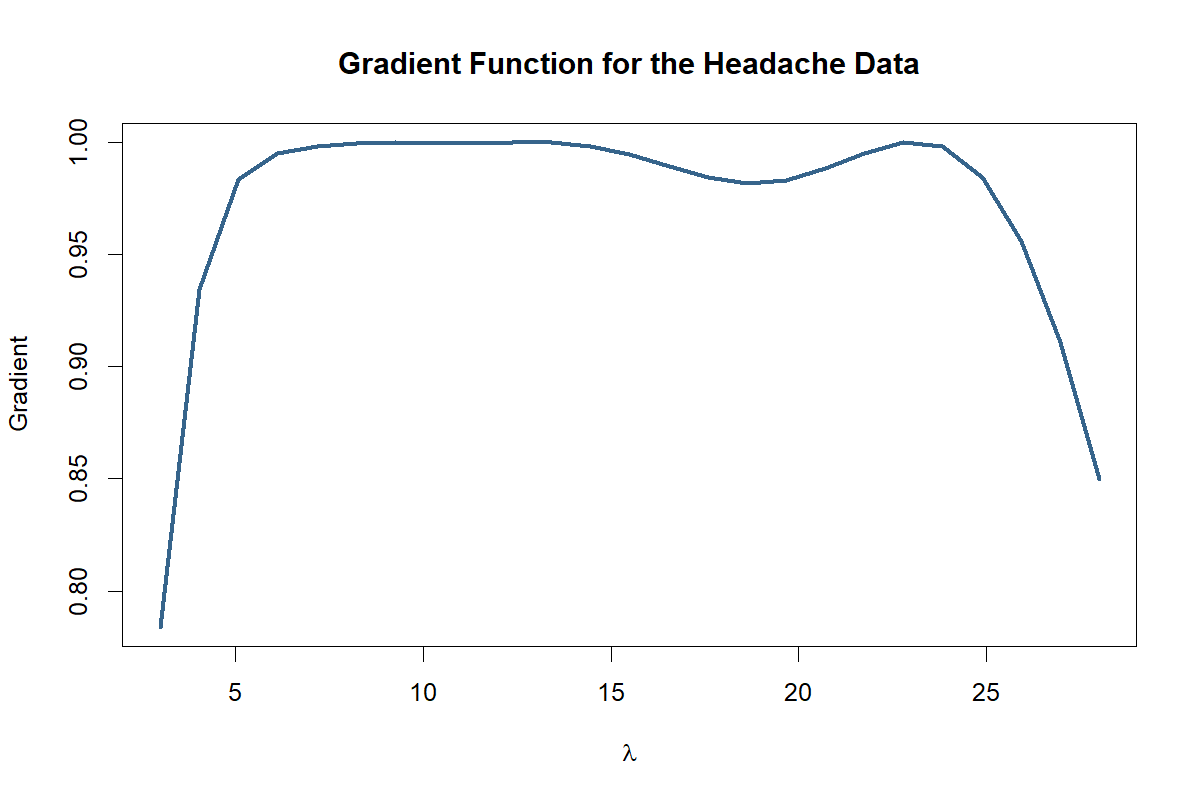
\includegraphics[width=0.85\textwidth]
{03_Output/gradient_function_npmle.png}
\caption{NPMLE gradient function for the baseline headache-frequency
data.}
\label{fig:gradient}
\end{figure}

The gradient function showed departures from a homogeneous
one-component structure and suggested the presence of multiple
regions in the underlying mixing distribution. This provided
exploratory support for fitting finite mixture models with more than
one component. The number of components was subsequently assessed
using fitted mixture models and information criteria.

%============================================================
\subsection{Comparison of Poisson Finite Mixture Models}
%============================================================

A single-component Poisson model was first fitted as a reference.
Two-, three-, four-, and five-component Poisson finite mixture
models were then fitted and compared using the Akaike Information
Criterion (AIC) and Bayesian Information Criterion (BIC).

\begin{table}[H]
\centering
\caption{Comparison of Poisson and finite mixture models}
\label{tab:modelcomparison}
\begin{tabular}{rrrr}
\toprule
Components & Log-Likelihood & AIC & BIC \\
\midrule
1 & -1476.032 & 2954.063 & 2958.057 \\
2 & -1309.058 & 2624.115 & 2636.097 \\
3 & -1306.585 & 2623.170 & 2643.140 \\
4 & -1306.585 & 2627.169 & 2655.127 \\
5 & -1306.548 & 2631.095 & 2667.041 \\
\bottomrule
\end{tabular}
\end{table}

The finite mixture models produced substantially lower AIC and BIC
values than the single-component Poisson model. The three-component
model had the lowest AIC (2623.170), whereas the two-component model
had the lowest BIC (2636.097).

The four- and five-component models did not provide a sufficient
improvement in model fit to compensate for their additional
complexity. The three-component model was therefore retained for
detailed interpretation because it provided the lowest AIC and
yielded three distinct and interpretable headache-frequency groups.

The difference between the AIC and BIC selections is important. The
results do not provide unanimous support for a single number of
components. Instead, AIC favored three components, while the more
strongly penalized BIC favored two components. The three-component
solution was therefore examined in greater detail as the principal
interpretable model.

%============================================================
\subsection{Three-Component Poisson Mixture Model}
%============================================================

The estimated parameters of the three-component Poisson mixture are
presented in Table~\ref{tab:threecomponent}. The component labels
reported by FlexMix are software-specific and are not ordered
according to headache frequency.

\begin{table}[H]
\centering
\caption{Estimated parameters of the three-component Poisson mixture}
\label{tab:threecomponent}
\begin{tabular}{rrrr}
\toprule
Frequency Group & $\lambda$ & Proportion & Patients \\
\midrule
Low-frequency & 9.61 & 0.2512 & 102 \\
Moderate-frequency & 13.80 & 0.3729 & 148 \\
High-frequency & 22.95 & 0.3759 & 151 \\
\bottomrule
\end{tabular}
\end{table}

The estimated component means indicate substantial differences in
baseline headache frequency. The low-frequency group had an
estimated mean of 9.61 headache days and represented 25.12\% of the
sample. The moderate-frequency group had an estimated mean of
13.80 days and represented 37.29\% of the sample. The high-frequency
group had the highest estimated mean, 22.95 days, and represented
37.59\% of the sample.

For interpretation, the three latent groups were therefore ordered
from lowest to highest estimated headache frequency as
low-frequency, moderate-frequency, and high-frequency groups.

The original FlexMix component labels are retained in the posterior
classification plot because the plot represents the component
assignments returned by the fitted model.

%============================================================
\subsection{Comparison of CAMAN and FlexMix Estimates}
%============================================================

The three-component solution was estimated independently using CAMAN
and FlexMix. The resulting estimates are compared in
Table~\ref{tab:camanflexmix}. Because mixture-component labels are
arbitrary and may differ between software implementations, the
comparison is based on the ordering of the estimated component means
rather than on the numerical component labels.

\begin{table}[H]
\centering
\caption{Comparison of CAMAN and FlexMix estimates by headache-frequency group}
\label{tab:camanflexmix}
\begin{tabular}{lrrrr}
\toprule
Frequency Group &
CAMAN $\lambda$ &
FlexMix $\lambda$ &
CAMAN Proportion &
FlexMix Proportion \\
\midrule
Low-frequency & 9.140 & 9.608 & 0.191 & 0.251 \\
Moderate-frequency & 13.334 & 13.804 & 0.427 & 0.373 \\
High-frequency & 22.895 & 22.950 & 0.382 & 0.376 \\
\bottomrule
\end{tabular}
\end{table}

The component means estimated by the two approaches were similar.
The absolute differences in the estimated means were 0.468, 0.470,
and 0.055 headache days for the low-, moderate-, and high-frequency
groups, respectively.

The estimated mixing proportions showed somewhat larger differences,
particularly for the low- and moderate-frequency groups. Nevertheless,
both approaches identified a similar three-level structure in the
headache-frequency distribution.

The close agreement between the estimated component means provides
support for the stability of the identified latent frequency groups
across the two R implementations.

%============================================================
\subsection{Posterior Classification of Patients}
%============================================================

Posterior probabilities from the three-component FlexMix model were
used to assign each patient to the component with the highest
posterior probability. The resulting classification separated the
patients into three groups corresponding to low-, moderate-, and
high-frequency headache patterns.

The posterior classification is presented in
Figure~\ref{fig:classification}.

\begin{figure}[H]
\centering
\includegraphics[width=0.95\textwidth]
{03_Output/posterior_classification_patients.png}
\caption{Posterior classification of patients under the
three-component Poisson finite mixture model. Points are coloured
according to the most likely latent component, with the estimated
component means displayed below the title.}
\label{fig:classification}
\end{figure}

The classification plot shows a clear separation of the three
estimated frequency groups. Patients assigned to the low-frequency
group were concentrated at lower headache frequencies, whereas the
high-frequency group contained patients with substantially more
headache days. The moderate-frequency group occupied an intermediate
range.

%============================================================
\subsection{Assessment of the Final Three-Component Model}
%============================================================

The fitted three-component model was further assessed by comparing
observed and expected frequencies across the headache-frequency
range.

\begin{table}[H]
\centering
\caption{Selected observed and expected frequencies under the
three-component model}
\label{tab:diagnostics}
\begin{tabular}{rrrr}
\toprule
Frequency & Observed & Expected & Pearson Residual \\
\midrule
3  & 2  & 1.067 & 0.903 \\
6  & 5  & 8.853 & -1.295 \\
10 & 33 & 23.159 & 2.045 \\
15 & 21 & 20.615 & 0.085 \\
20 & 13 & 15.030 & -0.524 \\
25 & 10 & 11.276 & -0.380 \\
27 & 10 & 8.311 & 0.586 \\
28 & 38 & 6.785 & 11.984 \\
\bottomrule
\end{tabular}
\end{table}

For most of the displayed frequencies, the observed and expected
counts were reasonably close. The main discrepancy occurred at the
upper boundary of 28 headache days. Thirty-eight patients were
observed at this value, compared with approximately 6.79 expected
under the fitted mixture. The resulting Pearson residual was 11.98.

This indicates substantial lack of fit at the upper boundary. Thus,
while the mixture model captured the main heterogeneous structure of
the data, it did not fully reproduce the concentration of patients
reporting the maximum observed number of headache days.

%============================================================
\subsection{Three-Component Model Including Age}
%============================================================

A three-component Poisson mixture model including age as a
covariate was subsequently fitted using SAS. The model had an AIC of
2612.2 and a BIC of 2644.2.

\begin{table}[H]
\centering
\caption{Age effects in the three-component Poisson mixture model}
\label{tab:ageeffects}
\begin{tabular}{rrrr}
\toprule
Component & Estimate & Standard Error & $p$-value \\
\midrule
1 & 0.002208 & 0.001975 & 0.2637 \\
2 & -0.024140 & 0.005593 & $<0.0001$ \\
3 & 0.003479 & 0.004569 & 0.4464 \\
\bottomrule
\end{tabular}
\end{table}

Age was statistically significant in SAS Component 2
($p<0.0001$). The estimated coefficient was negative
($\beta=-0.02414$). On the log scale, this corresponds to a
multiplicative change of

\[
\exp(-0.02414) \approx 0.976.
\]

Thus, within this component, a one-year increase in age was
associated with approximately a 2.4\% decrease in the expected
headache frequency.

The age effects for Components 1 and 3 were not statistically
significant. Their estimated coefficients were small and did not
provide sufficient evidence of an association between age and
headache frequency within those components.

Because latent-component labels can change between independently
fitted mixture models, SAS Component 2 is not assumed to correspond
directly to Component 2 in the earlier FlexMix model.

%============================================================
\subsection{Summary of Results}
%============================================================

The analysis showed substantial heterogeneity in baseline headache
frequency among the 401 patients. The variance-to-mean ratio of 2.78
indicated clear over-dispersion relative to the standard Poisson
model.

The NPMLE gradient analysis supported a heterogeneous mixing
distribution, and the finite mixture models provided substantially
lower information criteria than the single-component Poisson
reference model. AIC favored the three-component model, while BIC
favored two components. The three-component solution was examined
further because it provided the lowest AIC and produced three
interpretable headache-frequency groups.

The estimated mean headache frequencies for the three components
were 9.61, 13.80, and 22.95 days, with the groups representing
approximately 25\%, 37\%, and 38\% of the sample. Posterior
classification showed clear separation of patients across these
frequency levels.

The comparison between CAMAN and FlexMix produced similar
component-specific mean frequencies, although the estimated mixing
proportions differed between the two approaches. The final model
diagnostics showed that the mixture captured the broad structure of
the data but substantially underestimated the number of patients
reporting 28 headache days.

The age-adjusted analysis showed that the association between age and
headache frequency was not uniform across the latent population. Age
was statistically significant in one SAS component, with a negative
coefficient, whereas the effects in the other two components were
not statistically significant.